\documentclass[../../../main.tex]{subfiles}
\begin{document}

%%%%%%%%%%%%%%%%%%%%%%%%%%%%%%%%%%%%%%%%%
%%%%%%%%%%%%%%%%%%%%%%%%%%%%%%%%%%%%%%%%%
%%%%%%%%%%%%%%%%%%%%%%%%%%%%%%%%%%%%%%%%%
\chapter{Probability as area}


%%%%%%%%%%%%%%%%%%%%%%%%%%%%%%%%%%%%%%%%%
%%%%%%%%%%%%%%%%%%%%%%%%%%%%%%%%%%%%%%%%%
\section{Plotting \PDFtext/s}

\PDFtext/ functions assign probabilities to outcomes. They are useful because they let us look up the probability for a particular outcome.

We can plot \PDFtext/s too. For example, here is a \PDFtext/ table for flipping a coin:

\begin{center}
  \begin{tabular}{| l | l |}
    \hline
    \textbf{\RandVarVal/} & \textbf{\Probability{\RandVarVal/}} \\ \hline
    H & 0.5 \\ \hline
    T & 0.5 \\ \hline
  \end{tabular}
\end{center}

\noindent
We can plot this with a bar plot. For example:

\begin{center}
  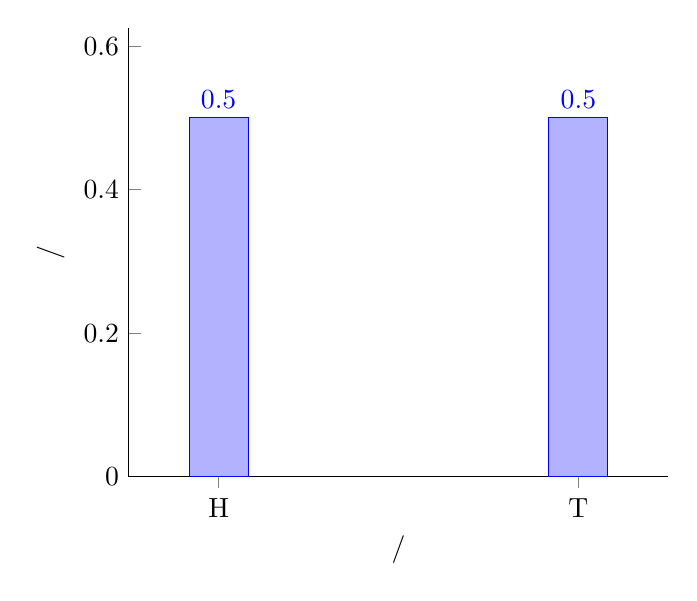
\begin{tikzpicture}
    % \centering
    \begin{axis} [
      axis lines*=left,
      ylabel=$\Probability{\RandVarVal/}$,
      xlabel=$\RandVarVal/$,
      symbolic x coords={H, T},
      ybar,
      xtick=data,
      ymin=0,
      enlarge y limits={value=0.25,upper},
      enlarge x limits=0.25,
      nodes near coords,
      bar width=0.75cm,
      ]
      \addplot coordinates {(H, 0.5) (T, 0.5)};
    \end{axis}
  \end{tikzpicture}
\end{center}

\noindent
In the plot, we can see that each outcome $\RandVarVal/$ is on the bottom axis, and the height of each bar (noted on the left axis) is the probability $\Probability{\RandVarVal/}$. And we can see that heads (H) has a probability of 0.5, and we can see that tails (T) also has a probability of 0.5. 

So this is a \vocab{uniform} distribution, because each possible outcome is equally likely (each outcome has the same probability). We can tell this because all of the bars are the same height.


%%%%%%%%%%%%%%%%%%%%%%%%%%%%%%%%%%%%%%%%%
\subsection{Line plot example 1}

We can also plot this \PDFtext/ as a line plot. For a line plot, we put dots at the top of the bars, and then draw a line through the points. So it looks like this:

\begin{center}
  \begin{tikzpicture}
    \begin{axis}[
      axis lines*=left,
      ylabel=$\Probability{\RandVarVal/}$,
      xlabel=$\RandVarVal/$,
      xtick=\empty,
      enlargelimits=false
      ]
      \addplot[domain=0:4] {0.5};
      \node[dot-point] at (axis cs:1, 0.5) [label=above:H] {};
      \node[dot-point] at (axis cs:3, 0.5) [label=above:T] {};
    \end{axis}
  \end{tikzpicture}
\end{center}

\noindent
Think about what the \PDFtext/ tells us here. A \PDFtext/ maps outcomes to probabilities. In the context of a line plot, we put the outcomes on the bottom axis, and then the probability for each outcome is how high up we draw the dot (i.e., probability is on the vertical axis). In this case, we have two outcomes --- H and T --- and in each case, the probability is 0.5, so we go up to 0.5 and draw a dot for each of them. Then we draw a line through the dots to show the shape.

The point here is this: in the context of a line plot, when we use a \PDFtext/ to look up the probability of an outcome, we are looking up its \vocab{height} on the line plot. So, when we put each point down and draw a line through them, the \PDFtext/ essentially tells us how to draw the \vocab{line} on the plot, and that line tells us the shape of the distribution.

Again, we can see that the distribution is uniform, because every probability is the same. We can tell because the line is flat. We don't have bars to show this, but the flat line tells us perfectly well that each outcome has the same probability.


%%%%%%%%%%%%%%%%%%%%%%%%%%%%%%%%%%%%%%%%%
\subsection{Line plot example 2}

Let's think about a distribution that's not uniform. Suppose we have a bag with five marbles in it, three of which are red, one of which is blue, and one of which is green. If you reach in the bag and pull out a marble, what are the probabilities of getting a red marble, a green marble, or a blue marble? The \PDFtext/ lookup table is this:

\begin{center}
  \begin{tabular}{| l | l |}
    \hline
    \textbf{\RandVarVal/} & \textbf{\Probability{\RandVarVal/}} \\ \hline
    R & 0.6 \\ \hline
    B & 0.2 \\ \hline
    G & 0.2 \\ \hline
  \end{tabular}
\end{center}

\noindent
If we put it into a line plot, we get this:

\begin{center}
  \begin{tikzpicture}
    \begin{axis}[
      axis lines*=left,
      ylabel=$\Probability{\RandVarVal/}$,
      xlabel=$\RandVarVal/$,
      xtick=\empty,
      enlarge x limits=false
      ]
      \addplot[domain=0:5] coordinates {(0, 0.6) (1, 0.6) (2, 0.2) (3, 0.2) (4, 0.2)};
      \node[dot-point] at (axis cs:1, 0.6) [label=above right:R] {};
      \node[dot-point] at (axis cs:2, 0.2) [label=above right:B] {};
      \node[dot-point] at (axis cs:3, 0.2) [label=above right:G] {};
    \end{axis}
  \end{tikzpicture}
\end{center}

\noindent
In this case, we can see that red (R) has a higher probability, because the line goes higher at that spot. So this is not a uniform distribution. One of the outcomes has a higher probability (is more likely) than the others.


%%%%%%%%%%%%%%%%%%%%%%%%%%%%%%%%%%%%%%%%%
\subsection{Line plot example 3}

Let's look at one more example of a line plot. We'll do another uniform distribution: rolling a (fair) six-sided die. The \PDFtext/ lookup table looks like this: 

\begin{center}
  \begin{tabular}{| l | l |}
    \hline
    \textbf{\RandVarVal/} & \textbf{\Probability{\RandVarVal/}} \\ \hline
    1 & 0.167 \\ \hline
    2 & 0.167 \\ \hline
    3 & 0.167 \\ \hline
    4 & 0.167 \\ \hline
    5 & 0.167 \\ \hline
    6 & 0.167 \\ \hline
  \end{tabular}
\end{center}

\noindent
And the line plot looks like this:

\begin{center}
  \begin{tikzpicture}
    \begin{axis}[
      axis lines*=left,
      ylabel=$\Probability{\RandVarVal/}$,
      xlabel=$\RandVarVal/$,
      xtick=\empty,
      enlargelimits=false
      ]
      \addplot[domain=0:7] {0.167};
      \node[dot-point] at (axis cs:1, 0.167) [label=above:1] {};
      \node[dot-point] at (axis cs:2, 0.167) [label=above:2] {};
      \node[dot-point] at (axis cs:3, 0.167) [label=above:3] {};
      \node[dot-point] at (axis cs:4, 0.167) [label=above:4] {};
      \node[dot-point] at (axis cs:5, 0.167) [label=above:5] {};
      \node[dot-point] at (axis cs:6, 0.167) [label=above:6] {};
    \end{axis}
  \end{tikzpicture}
\end{center}

\noindent
This is much like the line plot for the coin flip, except we have more outcomes. Here we have six outcomes, each with a probability of 0.167 (one-sixth). 


%%%%%%%%%%%%%%%%%%%%%%%%%%%%%%%%%%%%%%%%%
%%%%%%%%%%%%%%%%%%%%%%%%%%%%%%%%%%%%%%%%%
\section{More and more possible outcomes}

Let's plot the coin flip \PDFtext/ slightly differently. Let's do a bar plot, but let's draw a vertical line instead of a bar for each outcome:

\begin{center}
  \begin{tikzpicture}
    \begin{axis}[
      axis lines*=left,
      ylabel=$\Probability{\RandVarVal/}$,
      xlabel=$\RandVarVal/$,
      xtick=\empty,
      ytick={0.45, 0.5, 0.55},
      height=5cm,
      enlarge x limits=0.5,
      ybar,
      bar width=0cm
      ]
      \addplot[domain=0:4, color=gray] coordinates {(1, 0.5)(3, 0.5)};
      \node[dot-point] at (axis cs:1, 0.5) [label=above:H] {};
      \node[dot-point] at (axis cs:3, 0.5) [label=above:T] {};
    \end{axis}
  \end{tikzpicture}
\end{center}

\noindent
We can see that there are two outcomes here. Now consider a \PDFtext/ with more outcomes, like the six-sided die roll:

\begin{center}
  \begin{tikzpicture}
    \begin{axis}[
      axis lines*=left,
      ylabel=$\Probability{\RandVarVal/}$,
      xlabel=$\RandVarVal/$,
      xtick=\empty,
      height=5cm,
      width=10cm,
      % enlarge x limits=0.25,
      ybar,
      ytick={0.16},
      bar width=0cm
      ]
      \addplot[domain=0:7, color=gray] coordinates {(1, 0.16)(2, 0.16) (3, 0.16) (4, 0.16) (5, 0.16) (6, 0.16)};
      \node[dot-point] at (axis cs:1, 0.16) [label=above:1] {};
      \node[dot-point] at (axis cs:2, 0.16) [label=above:2] {};
      \node[dot-point] at (axis cs:3, 0.16) [label=above:3] {};
      \node[dot-point] at (axis cs:4, 0.16) [label=above:4] {};
      \node[dot-point] at (axis cs:5, 0.16) [label=above:5] {};
      \node[dot-point] at (axis cs:6, 0.16) [label=above:6] {};
    \end{axis}
  \end{tikzpicture}
\end{center}

\noindent
Notice that in both cases, the probability depends on how many points there are (i.e., how many outcomes there are).

\begin{itemize}
  \item For the coin flip, there are 2 outcomes. The total probability is always 1, and so if we divide that by 2, we get one-half, or 0.5.
  \item For the die roll, there are 6 outcomes. So if we divide 1 by six, we get one-sixth, or 0.167.
\end{itemize} 

\noindent
Imagine if there were even more outcomes. For example, 10 outcomes. Now the probability is one out of 10 (or 0.1):

\begin{center}
  \begin{tikzpicture}
    \begin{axis}[
      axis lines*=left,
      ylabel=$\Probability{\RandVarVal/}$,
      xlabel=$\RandVarVal/$,
      xtick=\empty,
      height=5cm,
      width=10cm,
      % enlarge x limits=0.25,
      ybar,
      ytick={0.1},
      bar width=0cm
      ]
      \addplot[domain=0:7, color=gray] coordinates {
        (0.5, 0.1) (1, 0.1)
        (1.5, 0.1) (2, 0.1) 
        (2.5, 0.1) (3, 0.1) 
        (3.5, 0.1) (4, 0.1) 
        (4.5, 0.1) (5, 0.1)
        };
      \node[dot-point] at (axis cs:0.5, 0.1) {};
      \node[dot-point] at (axis cs:1, 0.1) {};
      \node[dot-point] at (axis cs:1.5, 0.1) {};
      \node[dot-point] at (axis cs:2, 0.1) {};      
      \node[dot-point] at (axis cs:2.5, 0.1) {};
      \node[dot-point] at (axis cs:3, 0.1) {};
      \node[dot-point] at (axis cs:3.5, 0.1) {};
      \node[dot-point] at (axis cs:4, 0.1) {};
      \node[dot-point] at (axis cs:4.5, 0.1) {};
      \node[dot-point] at (axis cs:5, 0.1) {};
    \end{axis}
  \end{tikzpicture}
\end{center}

\noindent
Imagine 20 outcomes (each having a probability of one over 20, or 0.2):

\begin{center}
  \begin{tikzpicture}
    \begin{axis}[
      axis lines*=left,
      ylabel=$\Probability{\RandVarVal/}$,
      xlabel=$\RandVarVal/$,
      xtick=\empty,
      height=5cm,
      width=12cm,
      ybar,
      ytick=\empty,
      bar width=0cm
      ]
      \addplot[domain=0:3, color=gray] coordinates {
        (0.1, 0.01) (0.2, 0.01) (0.3, 0.01) (0.4, 0.01) (0.5, 0.01)
        (0.6, 0.01) (0.7, 0.01) (0.8, 0.01) (0.9, 0.01) (1, 0.01)
        (1.1, 0.01) (1.2, 0.01) (1.3, 0.01) (1.4, 0.01) (1.5, 0.01)
        (1.6, 0.01) (1.7, 0.01) (1.8, 0.01) (1.9, 0.01) (2, 0.01)
        };
      \node[dot-point] at (axis cs:0.1, 0.01) {};
      \node[dot-point] at (axis cs:0.2, 0.01) {};
      \node[dot-point] at (axis cs:0.3, 0.01) {};
      \node[dot-point] at (axis cs:0.4, 0.01) {};
      \node[dot-point] at (axis cs:0.5, 0.01) {};
      \node[dot-point] at (axis cs:0.6, 0.01) {};
      \node[dot-point] at (axis cs:0.7, 0.01) {};
      \node[dot-point] at (axis cs:0.8, 0.01) {};
      \node[dot-point] at (axis cs:0.9, 0.01) {};
      \node[dot-point] at (axis cs:1, 0.01) {};
      \node[dot-point] at (axis cs:1.1, 0.01) {};
      \node[dot-point] at (axis cs:1.2, 0.01) {};
      \node[dot-point] at (axis cs:1.3, 0.01) {};
      \node[dot-point] at (axis cs:1.4, 0.01) {};
      \node[dot-point] at (axis cs:1.5, 0.01) {};
      \node[dot-point] at (axis cs:1.6, 0.01) {};
      \node[dot-point] at (axis cs:1.7, 0.01) {};
      \node[dot-point] at (axis cs:1.8, 0.01) {};
      \node[dot-point] at (axis cs:1.9, 0.01) {};
      \node[dot-point] at (axis cs:2, 0.01) {};
    \end{axis}
  \end{tikzpicture}
\end{center}

\noindent
Imagine 100 outcomes (each having a probability of one over 100, or 0.01):

\begin{center}
  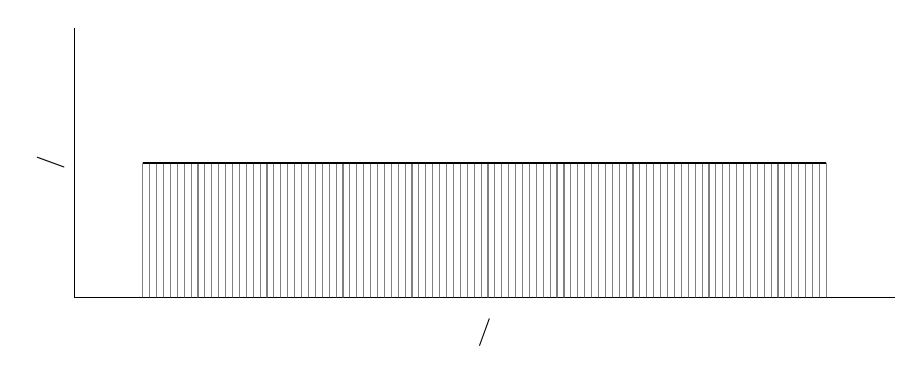
\begin{tikzpicture}
    \begin{axis}[
      axis lines*=left,
      ylabel=$\Probability{\RandVarVal/}$,
      xlabel=$\RandVarVal/$,
      xtick=\empty,
      height=5cm,
      width=12cm,
      ybar,
      ytick=\empty,
      bar width=0cm
      ]
      \addplot[domain=0:11, color=gray] coordinates {
        (0.1, 0.01) (0.2, 0.01) (0.3, 0.01) (0.4, 0.01) (0.5, 0.01)
        (0.6, 0.01) (0.7, 0.01) (0.8, 0.01) (0.9, 0.01) (1, 0.01)
        (1.1, 0.01) (1.2, 0.01) (1.3, 0.01) (1.4, 0.01) (1.5, 0.01)
        (1.6, 0.01) (1.7, 0.01) (1.8, 0.01) (1.9, 0.01) (2, 0.01)
        (2.1, 0.01) (2.2, 0.01) (2.3, 0.01) (2.4, 0.01) (2.5, 0.01)
        (2.6, 0.01) (2.7, 0.01) (2.8, 0.01) (2.9, 0.01) (3, 0.01)
        (3.1, 0.01) (3.2, 0.01) (3.3, 0.01) (3.4, 0.01) (3.5, 0.01)
        (3.6, 0.01) (3.7, 0.01) (3.8, 0.01) (3.9, 0.01) (4, 0.01)
        (4.1, 0.01) (4.2, 0.01) (4.3, 0.01) (4.4, 0.01) (4.5, 0.01)
        (4.6, 0.01) (4.7, 0.01) (4.8, 0.01) (4.9, 0.01) (5, 0.01)
        (5.1, 0.01) (5.2, 0.01) (5.3, 0.01) (5.4, 0.01) (5.5, 0.01)
        (5.6, 0.01) (5.7, 0.01) (5.8, 0.01) (5.9, 0.01) (6, 0.01)
        (6.1, 0.01) (6.2, 0.01) (6.3, 0.01) (6.4, 0.01) (6.5, 0.01)
        (6.6, 0.01) (6.7, 0.01) (6.8, 0.01) (6.9, 0.01) (7, 0.01)
        (7.1, 0.01) (7.2, 0.01) (7.3, 0.01) (7.4, 0.01) (7.5, 0.01)
        (7.6, 0.01) (7.7, 0.01) (7.8, 0.01) (7.9, 0.01) (8, 0.01)
        (8.1, 0.01) (8.2, 0.01) (8.3, 0.01) (8.4, 0.01) (8.5, 0.01)
        (8.6, 0.01) (8.7, 0.01) (8.8, 0.01) (8.9, 0.01) (9, 0.01)
        (9.1, 0.01) (9.2, 0.01) (9.3, 0.01) (9.4, 0.01) (9.5, 0.01)
        (9.6, 0.01) (9.7, 0.01) (9.8, 0.01) (9.9, 0.01) (10, 0.01)
        };
      \draw[thick] (0.1, 0.01) -- (10, 0.01);

    \end{axis}
  \end{tikzpicture}
\end{center}

\noindent
We can see here that, as the number of outcomes gets larger, we have to pack more and more of them into the space. So the sample space (the total shape) gets denser. 

We can also see that, as the number of outcomes gets larger, the probability gets smaller. And intuitively, this makes sense. As we add more and more outcomes to the plot, there are more ways the experiment can turn out, and so the chances of getting any one of them gets less and less. 

Now imagine a million outcomes (each with a probability of one over a million, or 0.000001). There are so many that the plot just looks like a grey square:

\begin{center}
  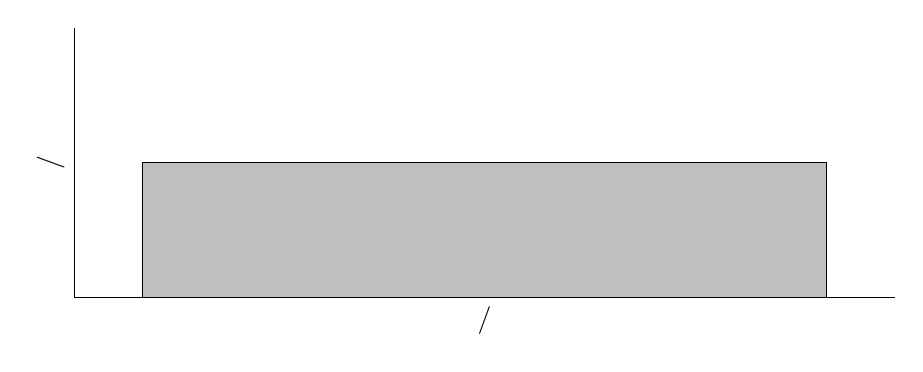
\begin{tikzpicture}
    \begin{axis}[
      axis lines*=left,
      ylabel=$\Probability{\RandVarVal/}$,
      xlabel=$\RandVarVal/$,
      ytick=\empty,
      xtick=\empty,
      height=5cm,
      width=12cm,
      ]
      \addplot[domain=0:11, fill=lightgray] {0.0000001} \closedcycle;
    \end{axis}
  \end{tikzpicture}
\end{center}

\noindent
This looks like a solid grey square, but the values are still discrete. If we zoomed in, we'd eventually start to see distinct vertical lines, like in the previous plots. Nevertheless, the point is obvious: as we add more and more outcomes, they get packed into the plot more and more densely.


%%%%%%%%%%%%%%%%%%%%%%%%%%%%%%%%%%%%%%%%%
\subsection{Individual probabilities get down to zero}

At this point, we can start to think about continuous values. Continuous values are infinitely dense. So, suppose we have not just a million vertical lines packed into the above plot, but rather an infinite number of them packed in there. 

Given that, ff the probability of any one outcome gets smaller as the number of outcomes increases, what happens when we have an \emph{infinite} number of outcomes? Well, the probability of any particular one of them gets so low, that it's practically zero. In fact, the probability of any one outcome in a set of infinite outcomes is one over infinity, which we treat as zero.
 
This may seem counterintuitive at first. A particular event has a probability of zero? But think about it. 

\begin{itemize}
  \item Think of flipping a coin. If you flip it again, what is the probability of getting the same result you got the first time? It's not too bad (the probability of flipping two of the same result is one in four).
  \item Think of rolling a (fair) six-sided die. Now think of rolling it again. What is the probability of getting the same result? Not as good as a coin flip, but not terrible (the probability of rolling the same thing twice is one in thirty-six).
  \item Imagine if there were such a thing as a (fair) 100-sided die. Suppose you roll it. If you roll it a second time, what is the probability of getting the same result? Now it seems much more unlikely (it's one in ten-thousand that you'll roll two of the same results with a 100-sided die).
  \item Imagine a (fair) one-million sided die. Suppose you roll it. Now, if you roll it a second time, what is the probability of rolling the same thing? It seems practically impossible that you would roll the same thing twice (the probability is one in a trillion). 
\end{itemize}

\noindent
If you have a million outcomes, the probability of getting any one of them is so incredibly small. So if you have an infinite number of possible outcomes, then surely the probability of getting any particular one of those is going to be so tiny that it's practically non-existent.


%%%%%%%%%%%%%%%%%%%%%%%%%%%%%%%%%%%%%%%%%
%%%%%%%%%%%%%%%%%%%%%%%%%%%%%%%%%%%%%%%%%
\section{Probability as area}

The above plots show that when we plot a continuous distribution, we end up with a solid shape:

\begin{center}
  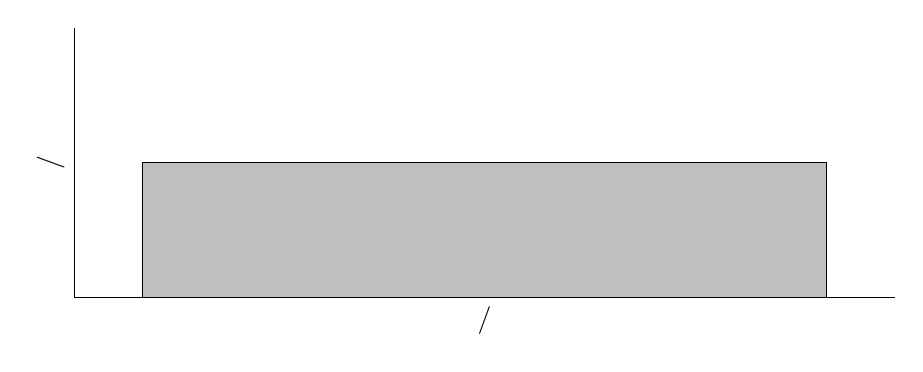
\begin{tikzpicture}
    \begin{axis}[
      axis lines*=left,
      ylabel=$\Probability{\RandVarVal/}$,
      xlabel=$\RandVarVal/$,
      ytick=\empty,
      xtick=\empty,
      height=5cm,
      width=12cm,
      ]
      \addplot[domain=0:11, fill=lightgray] {1} \closedcycle;
    \end{axis}
  \end{tikzpicture}
\end{center}

\noindent
Because the vertical lines that are packed into this distribution are \emph{infinitely} dense, this means that we can zoom in, and zoom in, and zoom in, and we can keep zooming in as long as we like, but we'll never see discrete vertical lines. We'll always see an infinitely dense solid wall of grey.

When we have continuous values, how do we deal with probability then? The answer is this: we think of probability as the shaded \vocab{area under the line}. 

We know that the total probability of all outcomes is always 1. So, let's say that the area under the line must be 1.

Then we can start talking about portions of the rectangle. For example, suppose we divide the rectangle in half:

\begin{center}
  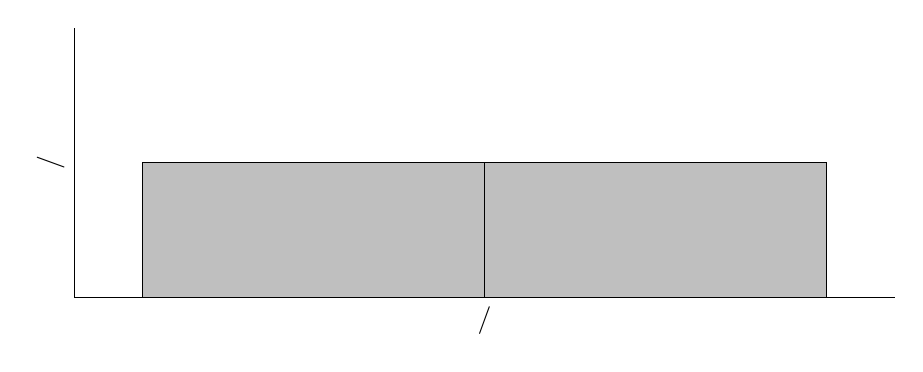
\begin{tikzpicture}
    \begin{axis}[
      axis lines*=left,
      ylabel=$\Probability{\RandVarVal/}$,
      xlabel=$\RandVarVal/$,
      ytick=\empty,
      xtick=\empty,
      height=5cm,
      width=12cm,
      ]
      \addplot[domain=0:11, fill=lightgray] {1} \closedcycle;
      \draw (5.5, 0) -- (5.5, 1);
    \end{axis}
  \end{tikzpicture}
\end{center}

\noindent
Since the whole shape has an area of 1, each of these halves must have an area of .5 each. Hence, half of the probability is on the left side:

\begin{center}
  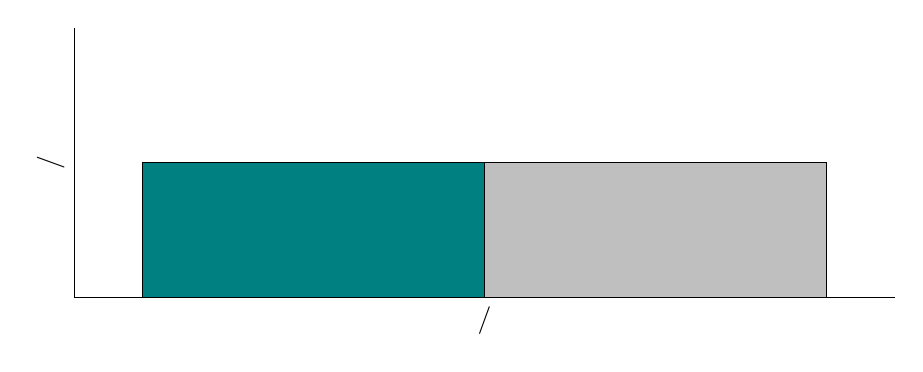
\begin{tikzpicture}
    \begin{axis}[
      axis lines*=left,
      ylabel=$\Probability{\RandVarVal/}$,
      xlabel=$\RandVarVal/$,
      ytick=\empty,
      xtick=\empty,
      height=5cm,
      width=12cm,
      ]
      \addplot[domain=0:11, fill=lightgray] {1} \closedcycle;
      \addplot[domain=0:5.5, fill=teal] {1} \closedcycle;
    \end{axis}
  \end{tikzpicture}
\end{center}

\noindent
And half is on the right side:

\begin{center}
  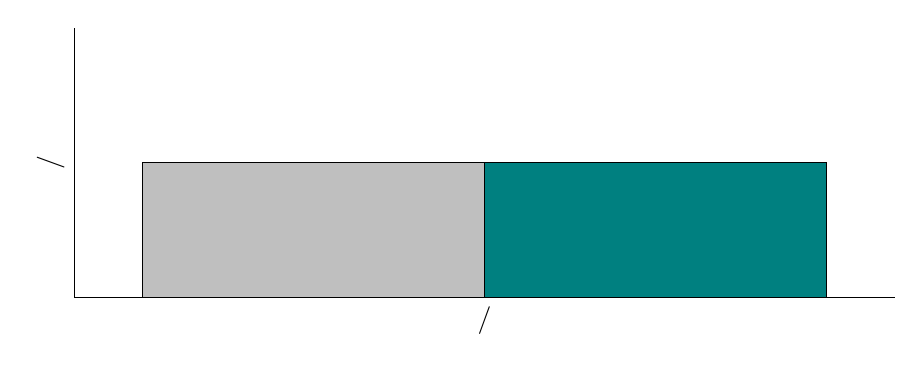
\begin{tikzpicture}
    \begin{axis}[
      axis lines*=left,
      ylabel=$\Probability{\RandVarVal/}$,
      xlabel=$\RandVarVal/$,
      ytick=\empty,
      xtick=\empty,
      height=5cm,
      width=12cm,
      ]
      \addplot[domain=0:11, fill=lightgray] {1} \closedcycle;
      \addplot[domain=5.5:11, fill=teal] {1} \closedcycle;
    \end{axis}
  \end{tikzpicture}
\end{center}

\noindent
Now, it doesn't make sense to ask for the exact probability of a \emph{particular} outcome, since the probability of any one outcome is zero, as we said. But it does make sense to ask about the probability of a \vocab{range} of values. 

For example, what is the probability of the range of outcomes that fall on the left side of the above plot? The probability is the area, so it is one-half, or 0.5. What is the probability of the range of outcomes that fall in the right hand side of the above plots? Again, it is one-half, or 0.5. 

We can make skinnier slices of the shape too. For example, here is a smaller range of outcomes:

\begin{center}
  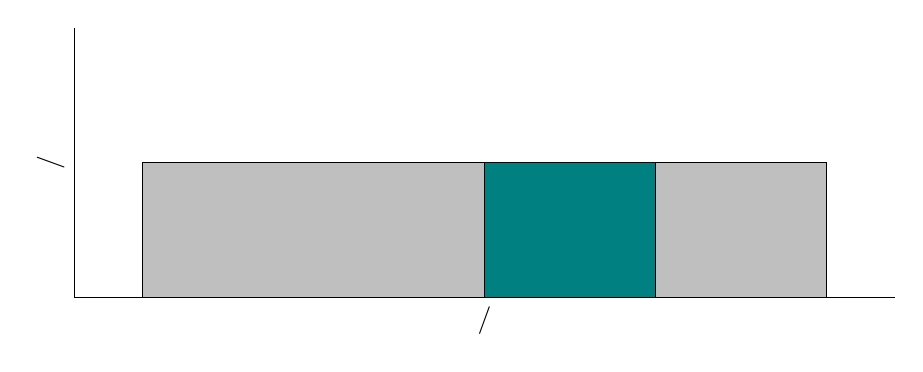
\begin{tikzpicture}
    \begin{axis}[
      axis lines*=left,
      ylabel=$\Probability{\RandVarVal/}$,
      xlabel=$\RandVarVal/$,
      ytick=\empty,
      xtick=\empty,
      height=5cm,
      width=12cm,
      ]
      \addplot[domain=0:11, fill=lightgray] {1} \closedcycle;
      \addplot[domain=5.5:8.25, fill=teal] {1} \closedcycle;
    \end{axis}
  \end{tikzpicture}
\end{center}

\noindent
What is the probability of this range? If you eyeball it, you can see that it's about one-fourth of the whole shape, so 0.25. 

In the above example, the line that is flat, so we have a rectangle shape. But sometimes the lines aren't flat, and they make different shapes. Here is one possible shape:

\begin{center}
  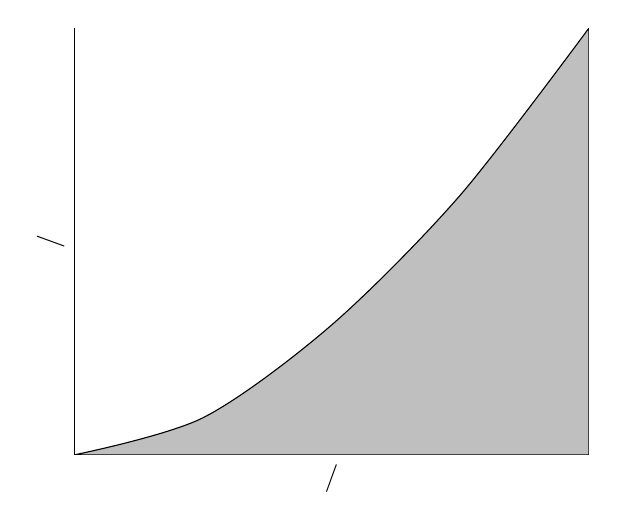
\begin{tikzpicture}
    \begin{axis}[
      axis lines*=left,
      ylabel=$\Probability{\RandVarVal/}$,
      xlabel=$\RandVarVal/$,
      ytick=\empty,
      xtick=\empty,
      height=7cm,
      enlargelimits=false
      ]
      \addplot[smooth, fill=lightgray] coordinates{(1, 2) (2, 4) (3, 9) (4, 16) (5, 25)} \closedcycle;
    \end{axis}
  \end{tikzpicture}
\end{center}

\noindent
The entire area of this shape is 1, since the total probability is always 1. We can also divide it in half. Half of the probability lies on the left side:

\begin{center}
  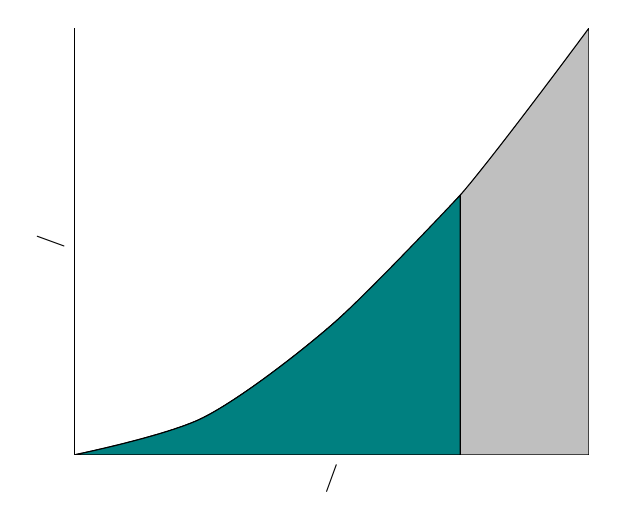
\begin{tikzpicture}
    \begin{axis}[
      axis lines*=left,
      ylabel=$\Probability{\RandVarVal/}$,
      xlabel=$\RandVarVal/$,
      ytick=\empty,
      xtick=\empty,
      height=7cm,
      enlargelimits=false
      ]
      \addplot[smooth, fill=lightgray] coordinates{(1, 2) (2, 4) (3, 9) (4, 16) (5, 25)} \closedcycle;
      \addplot[smooth, fill=teal] coordinates{(1, 2) (2, 4) (3, 9) (4, 16)} \closedcycle;
    \end{axis}
  \end{tikzpicture}
\end{center}

\noindent
And the other half of the probability lies on the right side:

\begin{center}
  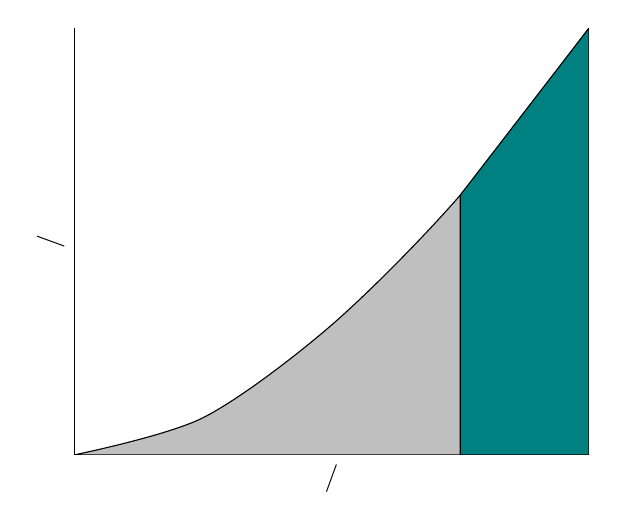
\begin{tikzpicture}
    \begin{axis}[
      axis lines*=left,
      ylabel=$\Probability{\RandVarVal/}$,
      xlabel=$\RandVarVal/$,
      ytick=\empty,
      xtick=\empty,
      height=7cm,
      enlargelimits=false
      ]
      \addplot[smooth, fill=lightgray] coordinates{(1, 2) (2, 4) (3, 9) (4, 16) (5, 25)} \closedcycle;
      \addplot[smooth, fill=teal] coordinates{(4, 16) (5, 25)} \closedcycle;
    \end{axis}
  \end{tikzpicture}
\end{center}

\noindent
So, to deal with probability with continuous values, we no longer ask for the probability of a \vocab{specific} outcome. Instead, we ask for the probability of a \vocab{range} of outcomes. And to calculate the probability of that range, we calculate the \vocab{area} of the shape under the line for that range. 


%%%%%%%%%%%%%%%%%%%%%%%%%%%%%%%%%%%%%%%%%
%%%%%%%%%%%%%%%%%%%%%%%%%%%%%%%%%%%%%%%%%
\section{Cumulative distribution functions}

A \PDFtext/ function maps outcomes to probabilities. When we plot it as a line graph, the \PDFtext/ function gives us the \vocab{line}. So the black line that we drew on top of the shape in the above drawings, the \PDFtext/ function gives us that line.

To calculate the area \emph{underneath} the line, we use a different function. We call that a \vocab{cumulative distribution function}, or \CDFtext/ for short. This is a function that maps \emph{ranges} of outcomes to probabilities. 


%%%%%%%%%%%%%%%%%%%%%%%%%%%%%%%%%%%%%%%%%
\subsection{Some notation}

With discrete values, the \PDFtext/ function gives us the point on the line for each outcome, and that point on the line \emph{is} the probability for that outcome. So we often write that the \PDFtext/ gives us $\Probability{\RandVarVal/}$.

For continuous values, the probability is not the point on the line. Instead, the probability is the area. So, we use $\Probability{\RandVarVal/}$ to refer to the \CDFtext/, not the \PDFtext/. 

But then we need a different symbol for the \PDFtext/, so when we are dealing with continuous values, we just write $\ContProb{\RandVarVal/}$. In summary:

\begin{itemize}
  \item For \vocab{discrete values}:
    \begin{itemize}
      \item $\Probability{\RandVarVal/}$ refers to the \PDFtext/.
    \end{itemize}
  \item For \vocab{continuous values}:
    \begin{itemize}
      \item $\ContProb{\RandVarVal/}$ refers to the \PDFtext/.
      \item $\Probability{\RandVarVal/}$ refers to the \CDFtext/.
    \end{itemize}
\end{itemize}


%%%%%%%%%%%%%%%%%%%%%%%%%%%%%%%%%%%%%%%%%
\subsection{What kind of function is a \CDFtext/?}

We know that, for continuous values, probability is area, so we can say that a \CDFtext/ function maps ranges of values to areas. Of course, there are an infinite number of ranges one could select out of any given set of continuous values, so there are too many rows to actually write down a full \CDFtext/ in the form of a lookup table, as we did with \PDFtext/s. 

Instead, we usually just write down a \CDFtext/ as a formula that one can use to compute a slice of the area under the line. 

Different \PDFtext/s give us differently shaped lines. For instance, uniform \PDFtext/s give us a flat line, but we just saw an example of a line that curves upwards. So the shape of the area under the line isn't always the same.

For each different kind of shape, we use a different \CDFtext/ formula, to calculate the area of that shape differently. For instance, for a rectangle, we can use the formula from geometry that we learned to calculate the area of a rectangle (base times height). But for a curve, we have to use something different.

To be fully general and calculate the area under \emph{any} curve, one would have to use calculus. But we will stick to shapes that don't require us to use calculus.


%%%%%%%%%%%%%%%%%%%%%%%%%%%%%%%%%%%%%%%%%
%%%%%%%%%%%%%%%%%%%%%%%%%%%%%%%%%%%%%%%%%
\section{Three common shapes}

Here are three examples of some common distribution shapes.

\begin{itemize}

  \item Here is a \vocab{uniform distribution} (with a portion of it highlighted), as we have seen already:
  
    \begin{center}
      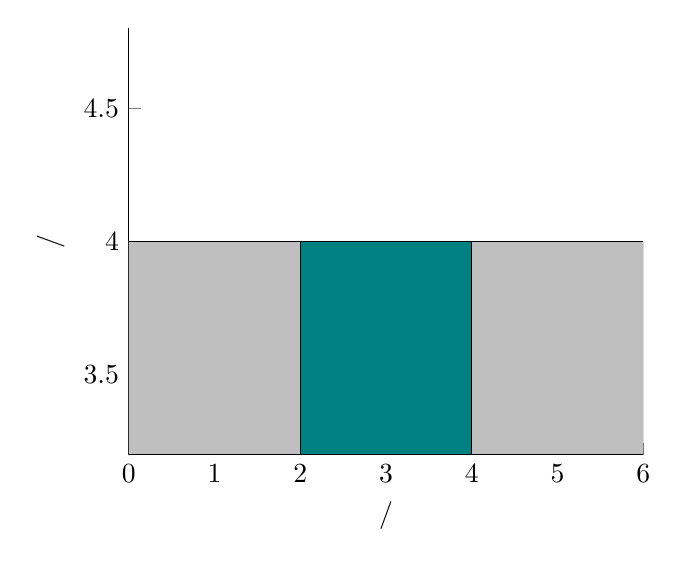
\begin{tikzpicture}
        \begin{axis}[
          no markers, % no dots
          axis lines*=left, % don't show axes on top and right
          ylabel=$\ContProb{\RandVarVal/}$,
          xlabel=$\RandVarVal/$,
          height=7cm,
          enlargelimits=false % don't put space around the curve
          ]
          \addplot[domain=0:6, samples=41, fill=lightgray] {4} \closedcycle;
          \addplot[domain=2:4, samples=41, fill=teal] {4} \closedcycle;
        \end{axis}
      \end{tikzpicture}
    \end{center}
    
    This distribution is always recognizable because it is a rectangle. The \PDFtext/ draws a flat line, which means that every outcome has the same probability. That is why we call it a \emph{uniform} distribution. The probabilities are divided up evenly (or you might say uniformly) amongst all possible outcomes.
  
  \item Here is an \vocab{exponential distirbution} (with a portion of it highlighted), as we have seen already:
  
    \begin{center}
      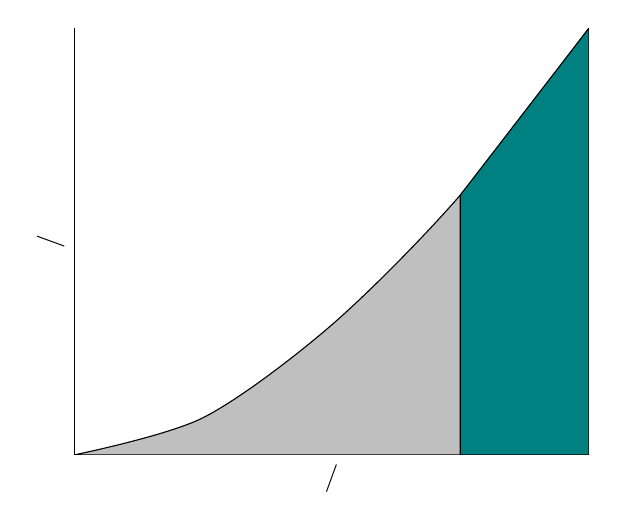
\begin{tikzpicture}
        \begin{axis}[
          axis lines*=left,
          ylabel=$\ContProb{\RandVarVal/}$,
          xlabel=$\RandVarVal/$,
          ytick=\empty,
          xtick=\empty,
          height=7cm,
          enlargelimits=false
          ]
          \addplot[smooth, fill=lightgray] coordinates{(1, 2) (2, 4) (3, 9) (4, 16) (5, 25)} \closedcycle;
          \addplot[smooth, fill=teal] coordinates{(4, 16) (5, 25)} \closedcycle;
        \end{axis}
      \end{tikzpicture}
    \end{center}
  
    In this shape, the probability gets higher and higher as we get towards the right side of the shape. The shape can go the other way too:
    
    \begin{center}
      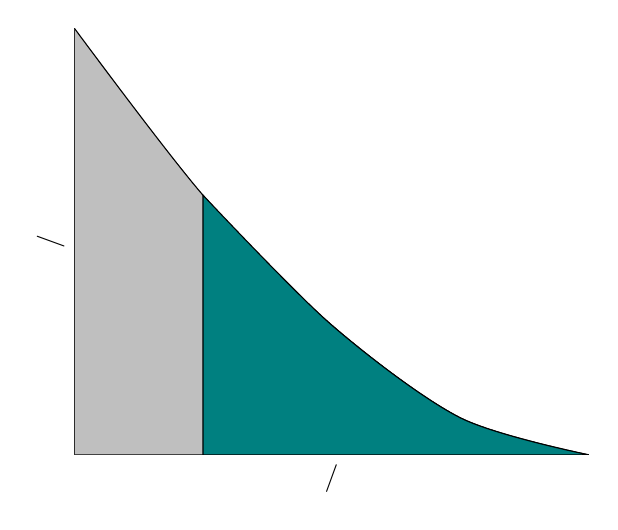
\begin{tikzpicture}
        \begin{axis}[
          axis lines*=left,
          ylabel=$\ContProb{\RandVarVal/}$,
          xlabel=$\RandVarVal/$,
          ytick=\empty,
          xtick=\empty,
          height=7cm,
          enlargelimits=false
          ]
          \addplot[smooth, fill=lightgray] coordinates{(1, 25) (2, 16) (3, 9) (4, 4) (5, 2)} \closedcycle;
          \addplot[smooth, fill=teal] coordinates{(2, 16) (3, 9) (4, 4) (5, 2)} \closedcycle;
        \end{axis}
      \end{tikzpicture}
    \end{center}
  
    This distribution is always recognizable because it always increases or decreases at a growing rate. We say it has an \emph{exponential} rate of growth (or decay). 
  
  \item Here is a \vocab{normal distribution} (with a portion of it highlighted):

    \begin{center}
      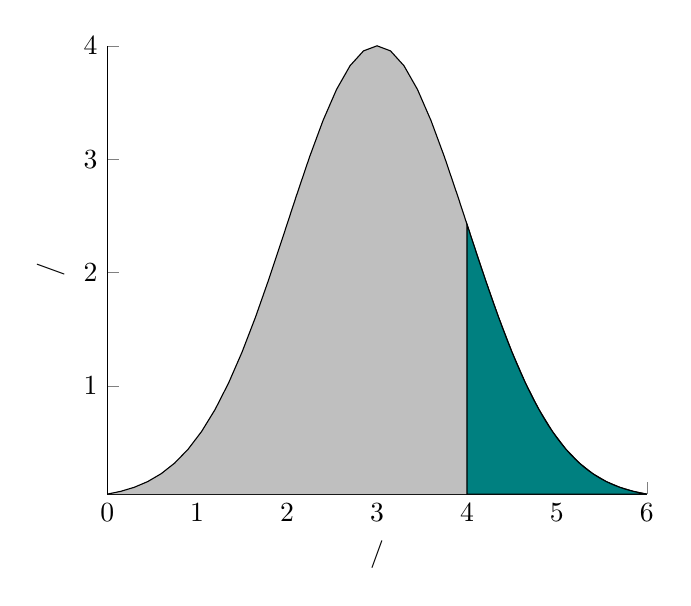
\begin{tikzpicture}
        \begin{axis}[
          no markers, % no dots
          axis lines*=left, % don't show axes on top and right
          ylabel=$\ContProb{\RandVarVal/}$,
          xlabel=$\RandVarVal/$,
          enlargelimits=false % don't put space around the curve
          ]
          \addplot[domain=0:6, samples=41, fill=lightgray] {4*1/exp(((x-3)^2)/2};
          \addplot[domain=4:6, samples=41, fill=teal] {4*1/exp(((x-3)^2)/2} \closedcycle;
        \end{axis}
      \end{tikzpicture}
    \end{center}

    This distribution is always recognizable because it has a distinctive bell curve shape.
    
\end{itemize}


\end{document}
